\documentclass{article}
\usepackage[margin=1in]{geometry}
\usepackage{titlesec}
\usepackage[hidelinks]{hyperref}
\usepackage{booktabs}
\usepackage{amsmath}
\usepackage{listings}
\usepackage{xcolor}
\usepackage{tikz}
\usepackage{capt-of}
\usetikzlibrary{arrows.meta, positioning, shapes.geometric}

\definecolor{codegreen}{rgb}{0,0.6,0}
\definecolor{codegray}{rgb}{0.5,0.5,0.5}
\definecolor{codepurple}{rgb}{0.58,0,0.82}
\definecolor{backcolour}{rgb}{0.95,0.95,0.92}

\lstdefinestyle{mystyle}{
    backgroundcolor=\color{backcolour},
    commentstyle=\color{codegreen},
    keywordstyle=\color{magenta},
    numberstyle=\tiny\color{codegray},
    stringstyle=\color{codepurple},
    basicstyle=\ttfamily\footnotesize,
    breakatwhitespace=false,
    breaklines=true,
    captionpos=b,
    keepspaces=true,
    numbers=left,
    numbersep=5pt,
    showspaces=false,
    showstringspaces=false,
    showtabs=false,
    tabsize=2
}
\lstset{style=mystyle}

% Style for shell scripts
\lstdefinestyle{shstyle}{
    language=bash,
    basicstyle=\ttfamily\footnotesize,
    keywordstyle=\color{blue},
    commentstyle=\color{codegreen},
    stringstyle=\color{codepurple},
    backgroundcolor=\color{backcolour},
    showstringspaces=false,
    numbers=left,
    numberstyle=\tiny\color{codegray},
    numbersep=5pt,
    breaklines=true,
    captionpos=b,
}

% Style for Python
\lstdefinestyle{pythonstyle}{
    language=Python,
    basicstyle=\ttfamily\footnotesize,
    keywordstyle=\color{blue},
    commentstyle=\color{codegreen},
    stringstyle=\color{codepurple},
    backgroundcolor=\color{backcolour},
    morekeywords={*,plt,pd,sys,os,re}, % Add common library names if needed
    showstringspaces=false,
    numbers=left,
    numberstyle=\tiny\color{codegray},
    numbersep=5pt,
    breaklines=true,
    captionpos=b,
}
% --- End Code Listing Styles ---


\title{Performance Impact of Garbage Collection in Real-World Applications}
\author{Lexo Liu}

\begin{document}

\begin{titlepage}
\centering
{\huge\bfseries Performance Impact of Garbage Collection in Real-World Applications\par}
\vspace{2cm}
{\large\bfseries How do performance characteristics vary between GC and non-GC languages?\par}
\vspace{1.5cm}
{\large Subject: Computer Science\par}
\end{titlepage}

\tableofcontents
\newpage


\section{Introduction}
\subsection{Memory Management in Programming}

Memory management is one of the fundamental challenges in systems and application programming. It determines how memory is allocated, used, and reclaimed during a program's execution. Mismanagement can lead to critical problems such as memory leaks, segmentation faults, or degraded performance. In most programming languages, memory can be divided into two major areas: \textbf{stack memory} and \textbf{heap memory}. These regions serve distinct purposes and are managed in fundamentally different ways. \textbf{Stack memory} is used to store function call frames, including local variables and return addresses. It follows a strict last-in, first-out (LIFO) order, meaning that memory is allocated when a function is called and deallocated automatically when the function returns. This behavior is managed by the compiler and operating system, making stack memory very efficient and deterministic. Importantly, programmers do not need to manually manage stack memory, and issues such as memory leaks or dangling pointers are extremely rare in stack-based memory. \textbf{Heap memory}, on the other hand, is used for dynamic memory allocation when the required lifetime of data is not bound to a function's scope. This memory must be manually allocated and deallocated using functions like \texttt{malloc()} and \texttt{free()} in C/C++. Failure to do so properly can lead to memory safety issues.

To simplify heap memory management and reduce such risks, many modern languages (e.g., Java, Go, Python) incorporate \textbf{garbage collection}, a form of automatic memory management that reclaims unused memory at runtime.

\begin{figure}[h]
\centering
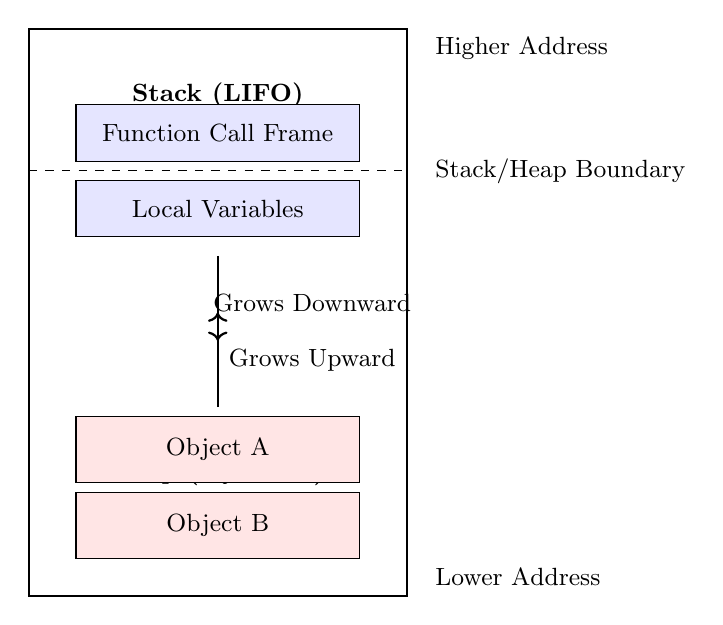
\begin{tikzpicture}[scale=1.2, every node/.style={font=\small}]
% Memory layout
\draw[thick] (0,0) rectangle (4,6);
\node[anchor=west] at (4.2,5.8) {Higher Address};
\node[anchor=west] at (4.2,0.2) {Lower Address};
% Stack region
\draw[dashed] (0,4.5) -- (4,4.5);
\node at (2,5.3) {\textbf{Stack (LIFO)}};
\draw[fill=blue!10] (0.5,4.6) rectangle (3.5,5.2);
\node at (2,4.9) {Function Call Frame};
\draw[fill=blue!10] (0.5,3.8) rectangle (3.5,4.4);
\node at (2,4.1) {Local Variables};
\draw[->, thick] (2,3.6) -- (2,2.7);
\node at (3,3.1) {Grows Downward};

% Heap region
\node at (2,1.3) {\textbf{Heap (Dynamic)}};
\draw[fill=red!10] (0.5,1.2) rectangle (3.5,1.9);
\node at (2,1.55) {Object A};
\draw[fill=red!10] (0.5,0.4) rectangle (3.5,1.1);
\node at (2,0.75) {Object B};
\draw[->, thick] (2,2.0) -- (2,3.0);
\node at (3,2.5) {Grows Upward};

% Label
\node[anchor=west] at (4.2,4.5) {Stack/Heap Boundary};
\end{tikzpicture}
\caption{Stack and Heap Memory Layout in a Typical Program }
\end{figure}

Understanding the differences between stack and heap memory is crucial for analyzing how programming languages manage memory. In the following sections, we will explore how heap memory is managed through manual techniques and automatic algorithms such as garbage collection.

\subsection{Research Motivation and Objectives}

Modern programming languages diverge significantly in their approach to memory management. While languages like C and Rust require manual memory management, offering fine-grained control at the cost of greater developer responsibility, languages like Java, Go, and Python implement automatic memory management through garbage collection. This fundamental difference raises important questions about the performance trade-offs between these approaches. This research aims to systematically investigate how garbage collection impacts application performance in real-world scenarios. While it is commonly accepted that automatic memory management introduces some overhead, the precise nature, extent, and practical implications of this overhead remain insufficiently documented across different types of applications and workloads. The primary objectives of this research are:

\begin{itemize}
    \item To quantify the performance differences between garbage-collected and manually managed languages in both compute-intensive and I/O-intensive tasks 
    \item To identify specific scenarios where garbage collection overhead is most significant 
    \item To analyze how modern garbage collection algorithms perform under different workload patterns 
    \item To provide evidence-based insights for developers making language selection decisions for performance-critical applications 
\end{itemize}

While previous studies have examined language performance differences, they often conflate multiple factors such as runtime environments, compiler optimizations, and language features. This research specifically isolates the impact of garbage collection by controlling for other variables and implementing algorithmically identical solutions across languages.


\section{Dynamic Memory Management: Evolution from Manual to Automatic}
\subsection{The Challenge of Manual Memory Management}

In the early days of programming, memory management was entirely manual. Languages such as C and C++ required programmers to explicitly control memory allocation and deallocation, providing precise control over system resources at the cost of increased development complexity. This manual approach requires programmers to allocate memory explicitly (using functions like \texttt{malloc} in C) and later free that memory when it is no longer needed (using \texttt{free}).

While manual memory management offers fine-grained control and potentially optimal performance, it introduces significant risks:

\begin{itemize}
    \item \textbf{Memory leaks} occur when allocated memory is never freed, gradually depleting available system resources.
    \item \textbf{Dangling pointers} arise when a program accesses memory that has already been freed, causing unpredictable behavior.
    \item \textbf{Double frees} happen when memory is deallocated multiple times, potentially corrupting memory management data structures.
    \item \textbf{Buffer overflows} result from writing beyond allocated memory boundaries, creating security vulnerabilities.
\end{itemize}

The prevalence of these errors in production software has driven the evolution toward safer memory management alternatives.

\subsubsection*{Manual Memory Management Examples in C}

\begin{lstlisting}[language=C, caption=Memory Leak Example, style=mystyle]
#include <stdlib.h>

void memory_leak() {
    int* data = (int*) malloc(100 * sizeof(int));
    // Function ends without freeing 'data'
    // This memory remains allocated but inaccessible
}
\end{lstlisting}

\begin{lstlisting}[language=C, caption=Dangling Pointer Example, style=mystyle]
#include <stdlib.h>
#include <stdio.h>

void dangling_pointer() {
    int* data = (int*) malloc(sizeof(int));
    *data = 42;
    free(data);
    // 'data' now points to invalid memory
    printf("%d\n", *data);  // Undefined behavior!
}
\end{lstlisting}

\subsection{The Evolution to Automatic Memory Management}

As software systems grew in complexity, the burden of manual memory management became increasingly problematic. This led to the development of automatic memory management techniques that could reliably handle memory allocation and deallocation without programmer intervention. Two primary approaches emerged: reference counting and tracing garbage collection.

\subsubsection{Reference Counting: A First Step}

Reference counting represents an intermediate step between manual and fully automatic memory management. In this approach, each allocated object maintains a counter that tracks how many references point to it:

\begin{itemize}
    \item When a new reference to an object is created, its reference count increments.
    \item When a reference is removed, the count decrements.
    \item When the count reaches zero, the object is automatically deallocated.
\end{itemize}

\begin{lstlisting}[language=Python, caption=Reference Counting Concept, style=pythonstyle]
def create_reference(obj):
    obj.ref_count += 1

def remove_reference(obj):
    obj.ref_count -= 1
    if obj.ref_count == 0:
        # Object has no more references
        for child in obj.references:
            remove_reference(child)  # Decrement children
        free(obj)  # Deallocate the object
\end{lstlisting}

While reference counting immediately reclaims memory when objects become unreachable and distributes collection overhead throughout program execution, it has a critical limitation: it cannot detect cyclic references.

\begin{figure}[h]
\centering
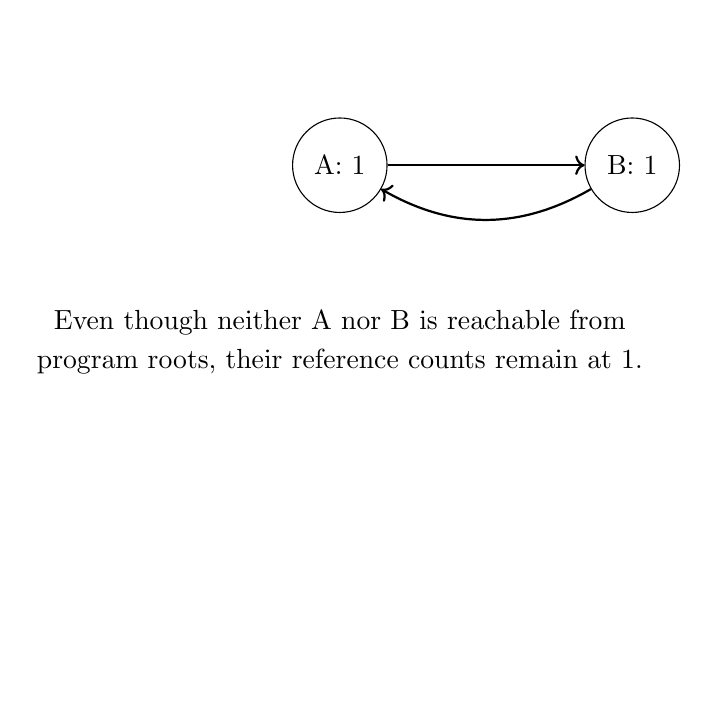
\begin{tikzpicture}[
  every node/.style={circle, draw, minimum size=1.2cm},
  node distance=2.5cm,
  arrow/.style={->, thick}
]
\node (A) {A: 1};
\node (B) [right=of A] {B: 1};

\draw[arrow] (A) -- (B) node[midway, above, draw=none] {};
\draw[arrow] (B) to [bend left=30] (A) node[midway, below, draw=none] {};

\node[draw=none] at (0,-2) {Even though neither A nor B is reachable from};
\node[draw=none] at (0,-2.5) {program roots, their reference counts remain at 1.};
\end{tikzpicture}
\caption{The cyclic reference problem: Objects A and B reference each other but are unreachable from program roots. Reference counting alone cannot detect this situation.}
\label{fig:cyclic_refs}
\end{figure}

As shown in Figure \ref{fig:cyclic_refs}, when objects form reference cycles, they may maintain non-zero reference counts even when the entire cycle is unreachable from the rest of the program. This results in memory leaks, undermining one of the primary benefits of automatic memory management.

\subsection{Tracing Garbage Collection: A Comprehensive Solution}

To address the limitations of reference counting, tracing garbage collection was developed based on a fundamentally different principle: \textbf{reachability analysis}. Rather than tracking individual references, tracing collectors determine whether objects are reachable from a set of root references within the program.

\subsubsection{Reachability Analysis: The Foundation of Modern GC}

In reachability analysis, memory can be modeled as a directed graph where:
\begin{itemize}
    \item Nodes represent allocated objects
    \item Edges represent references between objects
    \item Special nodes called "roots" represent references directly accessible to the program (e.g., global variables, stack variables, and registers)
\end{itemize}

The key insight of reachability analysis is that an object is "live" (still needed) if and only if it is reachable by following a path of references from any root. Conversely, any object that cannot be reached from the roots is definitionally unreachable by the program and can safely be reclaimed.

\begin{figure}[h]
\centering
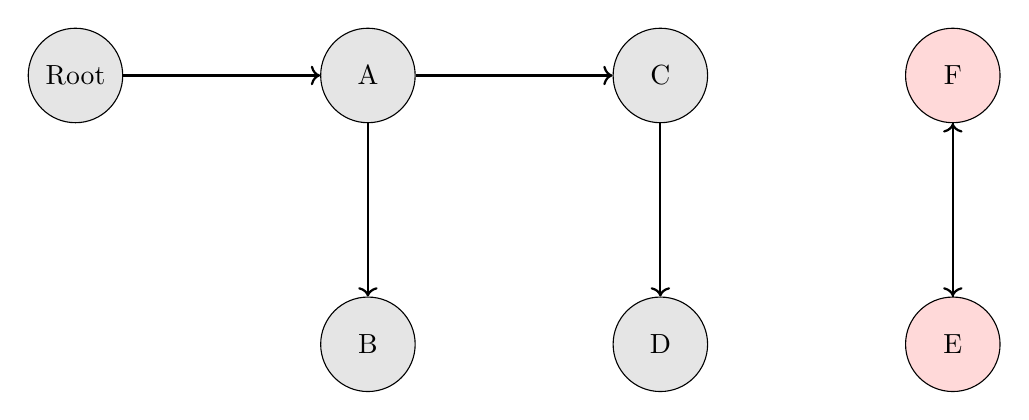
\begin{tikzpicture}[
  every node/.style={circle, draw, minimum size=1.2cm},
  node distance=2.2cm and 2.5cm,
  arrow/.style={->, thick},
  reachable/.style={fill=gray!20},
  unreachable/.style={fill=red!15}
]

\node[reachable] (root) {Root};
\node[reachable] (A) [right=of root] {A};
\node[reachable] (B) [below=of A] {B};
\node[reachable] (C) [right=of A] {C};
\node[reachable] (D) [below=of C] {D};
\node[unreachable] (E) [right=of D] {E};
\node[unreachable] (F) [right=of C] {F};

\draw[arrow] (root) -- (A);
\draw[arrow] (A) -- (B);
\draw[arrow] (A) -- (C);
\draw[arrow] (C) -- (D);
\draw[arrow] (E) -- (F);
\draw[arrow] (F) -- (E);

\end{tikzpicture}
\caption{Reachability analysis in garbage collection. Objects E and F form a cycle but are unreachable from any root, making them eligible for collection despite their mutual references.}
\label{fig:reachability}
\end{figure}

As illustrated in Figure \ref{fig:reachability}, reachability analysis elegantly solves the cyclic reference problem. Even though objects E and F reference each other (maintaining non-zero reference counts), they are unreachable from any root and therefore eligible for collection.

\subsubsection{Mark-and-Sweep: The Archetypal Tracing Algorithm}

The most fundamental tracing garbage collection algorithm is Mark-and-Sweep, which operates in two distinct phases:

\begin{itemize}
    \item \textbf{Mark Phase}: Starting from all roots, traverse the object graph and mark every object encountered as "reachable."
    \item \textbf{Sweep Phase}: Scan the entire heap and reclaim any unmarked objects, as they cannot be reached from the roots.
\end{itemize}

\begin{lstlisting}[language=Python, caption=Mark-and-Sweep Algorithm, style=pythonstyle]
def mark_and_sweep():
    # Mark phase
    for root in program_roots:
        mark(root)
    
    # Sweep phase
    for object in heap:
        if not object.is_marked:
            free(object)  # Object is unreachable, reclaim it
        else:
            object.is_marked = False  # Reset for next collection

def mark(object):
    if object is None or object.is_marked:
        return  # Already marked or null reference
    
    object.is_marked = True  # Mark as reachable
    
    # Recursively mark all referenced objects
    for reference in object.references:
        mark(reference)
\end{lstlisting}

The mark-and-sweep approach provides several advantages:
\begin{itemize}
    \item It correctly identifies and collects cyclic garbage
    \item It guarantees that all unreachable objects will be reclaimed
    \item It can be implemented efficiently with various optimizations
\end{itemize}

\section{The Performance Cost of Automatic Memory Management}
"No Silver Bullet" is a famous saying in computer science, it refers that there is no single thing could handle all condition perfectly without any cost. For manually memory allocation, the cost is convenience and safety. For reference counting, it is the risk of cyclic reference counting. And how about the cost for garbage collector?

From a theoretical perspective, garbage collection introduces several performance considerations:

\begin{itemize}
    \item \textbf{Stop-the-world pauses}: Traditional GC algorithms may temporarily halt program execution during collection phases, introducing latency spikes.
    \item \textbf{Memory overhead}: GC systems typically require more memory than manual management to operate efficiently, as they need space for bookkeeping and to amortize collection costs.
    \item \textbf{CPU overhead}: The collector consumes CPU cycles that could otherwise be used by the application logic.
    \item \textbf{Cache pollution}: GC operations may displace application data from CPU caches, affecting subsequent performance.
\end{itemize}

\section{Literature Review}
\subsection{Language Selection}
Initially, Java, Rust, and Go were selected to represent different memory management strategies: manual (Rust), garbage-collected (Go), and virtual machine-based GC (Java). However, benchmark results revealed that Java suffered severe performance degradation in short-lived compute tasks due to JVM warmup overhead and uncontrollable GC behavior.

Despite multiple warmup attempts, Java's performance was over 10x worse than Go or Rust in compute benchmarks (see Figure~\ref{fig:fib_java}). Due to these confounding variables, Java was excluded from the final analysis to ensure a fair and focused comparison between two compiled languages: Rust and Go.

\begin{table}[h]
\centering
\begin{tabular}{@{}lll@{}}
\toprule
Language & Memory Management & Compilation Model \\
\midrule
Rust     & Manual             & Native (AOT) \\
Go       & Garbage Collected  & Native (AOT) \\
\bottomrule
\end{tabular}
\caption{Languages selected for final comparison}
\end{table}

\section{Experimental Framework}
To systematically evaluate the performance impact of garbage collection across different workloads and platforms, a modular and reproducible experimental framework was designed and implemented. This framework provides the necessary infrastructure for compiling source code, running benchmarks consistently, and collecting performance data.

\subsection{Framework Architecture}

The benchmark system is organized within a top-level directory named `Benchmark/`. This directory contains the core automation scripts, specific benchmark implementations categorized by workload type, and tooling for data analysis and visualization.

\subsubsection{Directory Structure}
The framework employs a hierarchical structure to organize benchmark tasks:
\begin{itemize}
    \item \textbf{Benchmark/}: The root directory containing automation scripts and subdirectories for benchmark categories.
    \item \textbf{Compute/}: Contains subdirectories for CPU-intensive tasks. Each subdirectory (e.g., `FibonacciLoop/`, `Matrix/`, `Pi/`) holds the language-specific implementations (Go, Java, Rust) for that compute task.
    \item \textbf{IO/}: Contains subdirectories for I/O-bound tasks, such as `LargeFile/` for file operations and `WebServer/` for simulating network request handling. Similar to `Compute/`, each task directory contains the respective language implementations.
\end{itemize}
This modular organization facilitates the addition of new benchmark tasks or language implementations. A visual representation of the structure is shown in Figure \ref{fig:framework-structure}.

\begin{figure}[h!]
\centering
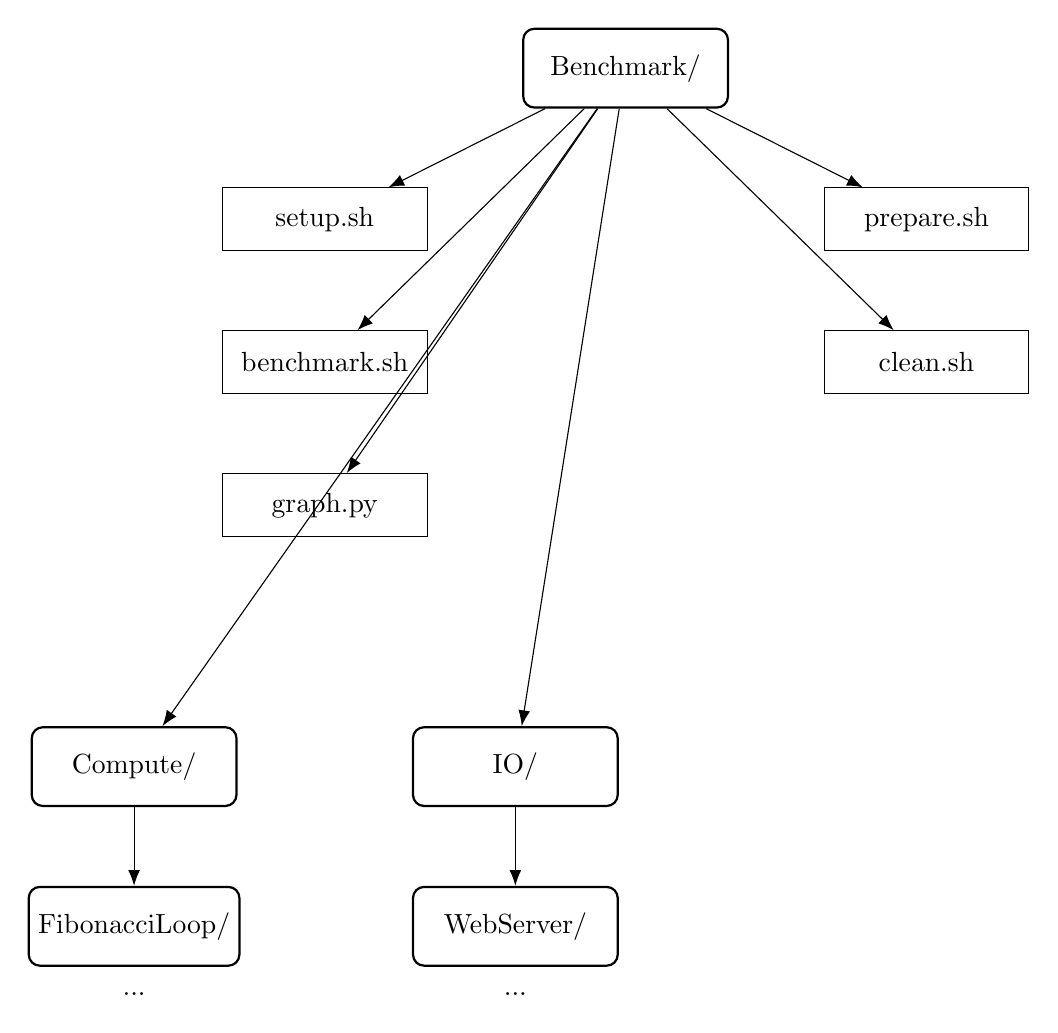
\begin{tikzpicture}[
  node distance=1cm and 1.2cm,
  folder/.style={draw, thick, minimum width=2.6cm, minimum height=1cm, text centered, rounded corners},
  script/.style={draw, minimum width=2.6cm, minimum height=0.8cm, text centered},
  line/.style={draw, -{Latex[length=2mm]}}
]

% Top node
\node (benchmark) [folder] {Benchmark/};

% First layer scripts
\node (setup)   [script, below left=of benchmark] {setup.sh};
\node (prepare) [script, below right=of benchmark] {prepare.sh};

% Second layer: benchmark & clean scripts
\node (benchsh) [script, below=of setup] {benchmark.sh};
\node (cleansh) [script, below=of prepare] {clean.sh};

% graph.py
\node (graph) [script, below=of benchsh] {graph.py};

% Compute & IO folders
\node (compute) [folder, below left=2.4cm and -0.2cm of graph] {Compute/};
\node (io)      [folder, below right=2.4cm and -0.2cm of graph] {IO/};

% Subfolders in Compute and IO
\node (fib) [folder, below=of compute] {FibonacciLoop/};
\node (web) [folder, below=of io] {WebServer/};

\node (fibdots) [below=0.2cm of fib] {...};
\node (webdots) [below=0.2cm of web] {...};

% Connections
\draw [line] (benchmark) -- (setup);
\draw [line] (benchmark) -- (prepare);
\draw [line] (benchmark) -- (benchsh);
\draw [line] (benchmark) -- (cleansh);
\draw [line] (benchmark) -- (graph);
\draw [line] (benchmark) -- (compute);
\draw [line] (benchmark) -- (io);
\draw [line] (compute) -- (fib);
\draw [line] (io) -- (web);

\end{tikzpicture}
\caption{High-level structure of the benchmark framework.}
\label{fig:framework-structure}
\end{figure}

\subsubsection{Automation Scripts}
A set of shell scripts automates the benchmarking workflow, ensuring consistency and reproducibility:
\begin{itemize}
    \item \texttt{setup.sh}: Prepares the testing environment by installing necessary dependencies such as the Rust compiler, Go compiler, Java Development Kit (JDK), and the `hyperfine` benchmarking tool. It includes OS detection for compatibility with macOS and Linux.
    \item \texttt{prepare.sh}: Compiles all Go, Java, and Rust source files found within the task subdirectories, creating executable binaries or class files. Optimization flags are used for compiled languages (e.g., `rustc -O` or `rustc -C opt-level=3`).
    \item \texttt{benchmark.sh}: Executes the core benchmarking logic for a specified task directory. It utilizes the `hyperfine` tool to run the compiled programs, collect timing data, perform statistical analysis (mean, standard deviation), handle warmup runs, and export results to CSV and Markdown formats.
    \item \texttt{run.sh}: A helper script, typically invoked by `hyperfine` within `benchmark.sh`, responsible for executing a specific language's compiled program for a given task.
    \item \texttt{clean.sh}: Removes compiled artifacts (executables, `.class` files) to ensure a clean state before subsequent runs.
    \item \texttt{graph.py}: A Python script that reads the CSV output generated by `hyperfine` and uses `matplotlib` and `pandas` to create bar charts visualizing the mean execution times for each language within a benchmark task, saving them as PNG images.
\end{itemize}

\subsection{Benchmarking Tool: Hyperfine}

The framework relies on \texttt{hyperfine}, a command-line benchmarking tool chosen for its robustness and features suitable for this research. Key capabilities leveraged include:
\begin{itemize}
    \item \textbf{Statistical Analysis}: Automatically computes mean, median, standard deviation, minimum, and maximum execution times over multiple runs.
    \item \textbf{Warmup Runs}: Allows specifying a number of initial runs (\texttt{--warmup N}) whose results are discarded, mitigating skewed measurements due to initial setup costs like JIT compilation or cache population.
    \item \textbf{Run Count}: Enables setting the number of measured runs (\texttt{--runs N}) for statistical significance.
    \item \textbf{Output Formats}: Exports results in various formats, including CSV for data analysis and Markdown for easy reporting.
    \item \textbf{Inter-process Measurement}: Accurately measures the wall-clock time of external commands.
\end{itemize}
A typical invocation within the framework looks like this:
\begin{lstlisting}[language=bash, caption={Example hyperfine usage in benchmark.sh }, style=shstyle]
hyperfine \
  --warmup 3 \
  --runs 10 \
  --export-csv "benchmark_TASK.csv" \
  --export-markdown "benchmark_TASK.md" \
  "./Rust_TASK <args>" \
  "./Go_TASK <args>" \
  "java Java_TASK <args>" # Example, actual execution might use run.sh
\end{lstlisting}

\subsection{Cross-Platform Testing} % Retained from original, slightly rephrased

The framework is designed to be executed on diverse hardware architectures to assess how performance characteristics, particularly those related to GC, might vary:
\begin{itemize}
    \item Personal computer (e.g., Macbook Pro) 
    \item Cloud-based server (e.g., Linux server, x86 architecture) 
    \item Embedded platform (e.g., ESP32, representing resource-constrained devices) 
\end{itemize}
This multi-platform testing strategy aims to provide a broader understanding of GC performance implications across different computational scales and constraints.


\section{Methodology}

\subsection{Benchmark Types and Design Philosophy}

The experiment employs two categories of benchmarks inspired by engineering experimental approaches:

\begin{itemize}
    \item \textbf{Micro-benchmarks (Compute-bound)}: These tests focus on specific computational algorithms implemented identically across languages (e.g., calculating Fibonacci numbers iteratively/recursively, matrix multiplication, Pi computation ). They are designed to stress CPU and memory subsystems under controlled conditions, making it easier to observe the direct impact of language runtime and GC on raw computation speed.
    \item \textbf{Simulated Workloads (I/O-bound / Mixed)}: These benchmarks aim to mimic aspects of real-world applications, involving both computation and significant I/O operations (e.g., reading/writing large files, simulating basic web server request handling ). They provide insights into performance under more complex, less predictable conditions where factors like I/O latency, concurrency, and GC behavior during idle or busy periods interact.
\end{itemize}
This dual approach allows for both focused analysis of specific performance aspects (computation, memory allocation frequency) and evaluation under more holistic, application-relevant scenarios.

\subsection{Implementation Strategy}

All benchmark algorithms are implemented from scratch within the respective language subdirectories (e.g., `Compute/FibonacciLoop/FibonacciLoop.go`, `Compute/FibonacciLoop/FibonacciLoop.rs`, etc.). Crucially, only the standard libraries native to each language (Go standard library, Rust std, Java standard libraries) are utilized. This constraint minimizes the influence of third-party library performance differences and ensures that the core comparison centers on the language's runtime, compiler, and memory management strategy (manual vs. GC). The algorithmic logic for each benchmark task is kept identical across language implementations.

\subsection{Testing Platforms} % Combined with section 5.5

The benchmarks are executed on the three distinct platforms previously mentioned (Macbook, x86 Server, ESP32) to analyze performance across varying hardware capabilities, including CPU architecture, core count, memory size, and speed. This helps determine if the relative performance characteristics and GC impact observed are consistent or platform-dependent.


\section{Results \& Analysis}
\subsection{Benchmark 1: Pi Computation}
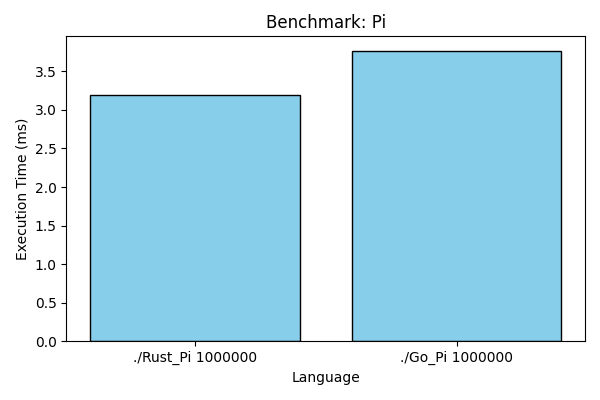
\includegraphics[width=0.5\textwidth]{../Benchmark/Compute/Pi/benchmark_Pi.png}
\captionof{figure}{Execution time for Pi computation (1,000,000 iterations)}
Rust completed the task in 3.2 ms and Go in 3.8 ms. Despite Rust's use of LLVM and manual memory, Go's GC overhead remained negligible in this compute-heavy task.

\subsection{Benchmark 2: Fibonacci Loop}
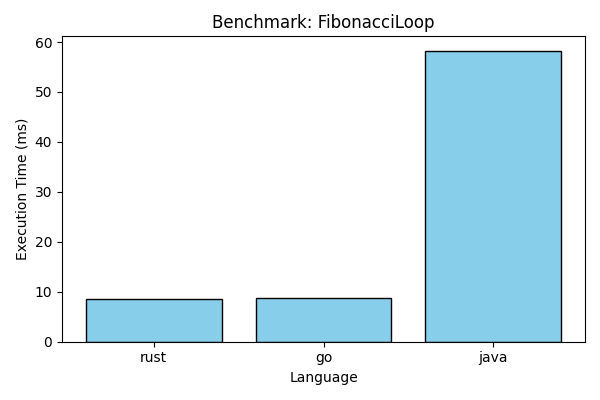
\includegraphics[width=0.5\textwidth]{../Benchmark/Compute/FibonacciLoop/benchmark_FibonacciLoop.png}
\captionof{figure}{Iterative Fibonacci computation: Rust vs Go vs Java}
Rust and Go completed in under 9 ms, whereas Java took nearly 58 ms, motivating its removal from further analysis.

\subsection{Benchmark 3: Recursive Fibonacci}
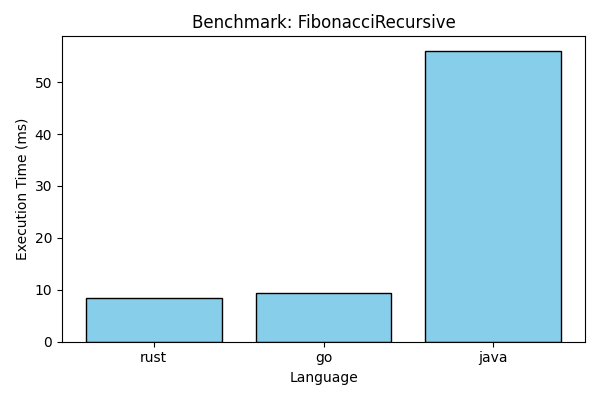
\includegraphics[width=0.5\textwidth]{../Benchmark/Compute/FibonacciRecursive/benchmark_FibonacciRecursive.png}
\captionof{figure}{Recursive Fibonacci: Rust vs Go vs Java}
Again, Rust and Go performed closely (within 1 ms), showing consistent parity in CPU-bound workloads.

\subsection{Findings Summary}
These results challenge assumptions that garbage collection inherently causes significant slowdowns. In compute-dense workloads with minimal heap allocation, Go performs nearly as well as Rust.

\section{Discussion}
While Rust's compile-time memory guarantees and zero-cost abstractions make it ideal for predictable performance, Go demonstrates that well-engineered garbage collectors can remain competitive, especially when memory pressure is low. The marginal performance difference suggests that memory management strategy is only one factor among many, including runtime design, compiler optimizations, and allocation patterns.

In real-world compute tasks, GC-induced pauses are less significant than expected, especially when allocation rates are low. This finding aligns with Go's design philosophy, which encourages allocation-free code for performance-sensitive sections.

\section{Conclusion}
This research evaluated the performance trade-offs between garbage-collected (Go) and manually-managed (Rust) languages using real-world compute benchmarks. The experimental evidence suggests that:

\begin{itemize}
  \item Garbage collection overhead is negligible in compute-intensive scenarios with low allocation frequency
  \item Rust offers better theoretical control but does not always yield drastic performance gains
  \item Go provides sufficient performance for many real-world tasks, simplifying development without major cost
\end{itemize}

Future work may extend to IO-bound and concurrency-heavy scenarios, where memory pressure and GC activity are more variable.

\section{References}
% Use BibTeX or manual references in APA style

\section{Appendices}
% Benchmark data tables, additional charts, scripts

\end{document}
